\begin{frame}[t]
\frametitle{Impact on communication}
  \begin{itemize}
    \item Current use of communication network
    \begin{itemize}
      \item Compute-communicate cycles in typical MPI apps
      \item Network is used for a fraction of time
      \item And is on the critical path
    \end{itemize}
    \pause
    \item Hence, current communication networks are over-engineered by necessity
    \pause
    \item With overdecomposition
    \begin{itemize}
      \item Communication is spread over an iteration
      \item Adaptive overlap of communication and computation
    \end{itemize}
  \end{itemize}
\end{frame}

\begin{frame}[t]
\frametitle{Example: Stencil Computation}
  \begin{itemize}
    \item Consider a simple stencil computation
    \begin{itemize}
      \item With traditional design based on traditional methods (e.g.  MPI-based)
      \begin{itemize}
        \item Each processor has a chunk, which alternates between computing and communicating
      \end{itemize}
      \pause
      \item With Charm++
      \begin{itemize}
        \item Multiple chunks on each processor
        \item Wait time for each chunk overlapped with useful computation for others
        \item Communication spread over time
      \end{itemize}
    \end{itemize}
  \end{itemize}
\end{frame}

\begin{frame}[t]
\frametitle{Example: Stencil Computation}
  \begin{center} 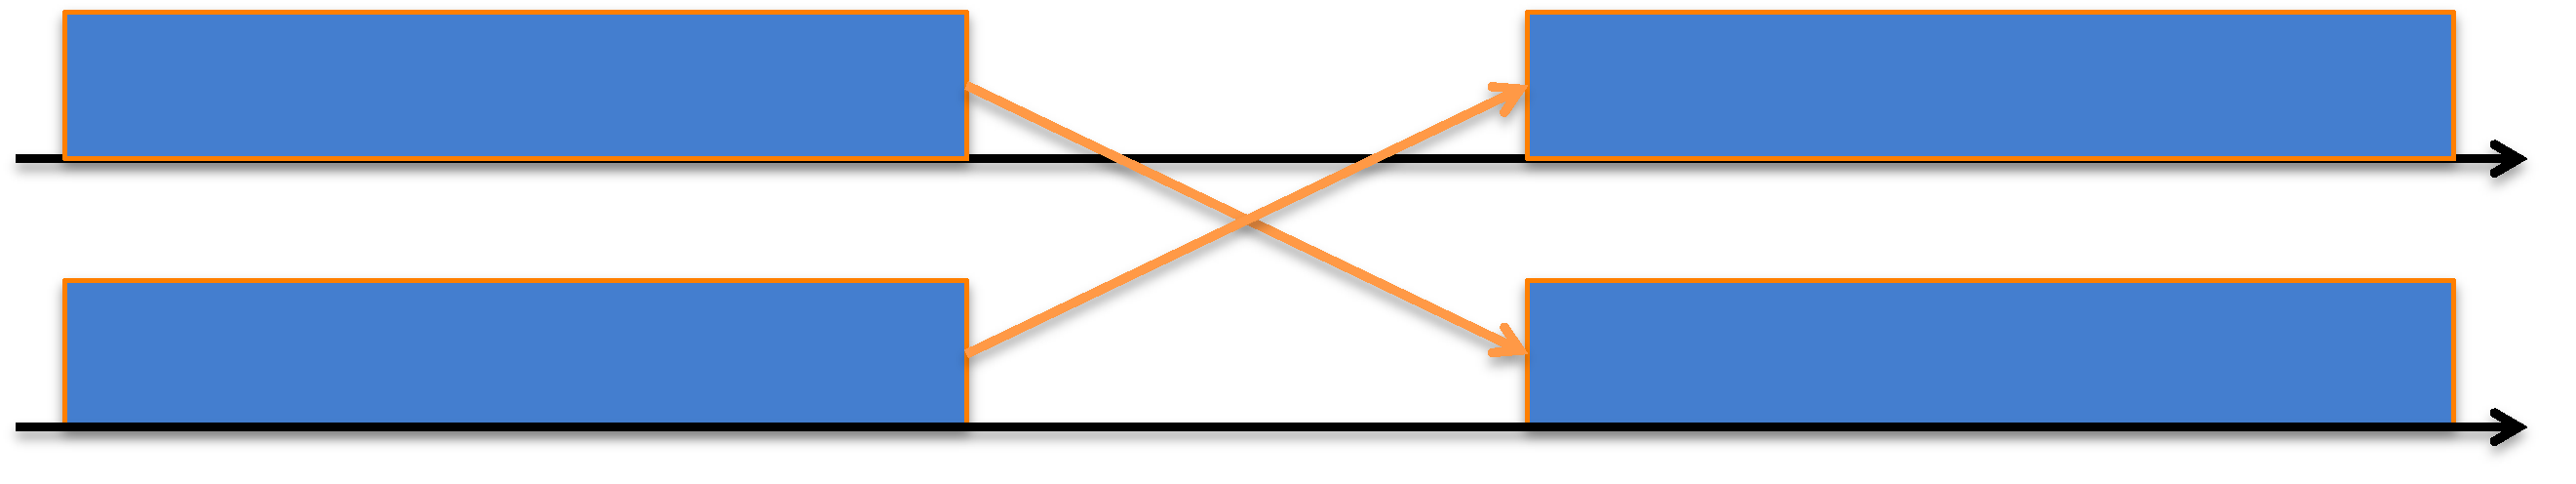
\includegraphics[width=\textwidth]{figures/stencil_timeline} \end{center}
  \begin{center} Stencil in MPI: No overlap among computation and
  communication\end{center}
  \pause
  \begin{center} 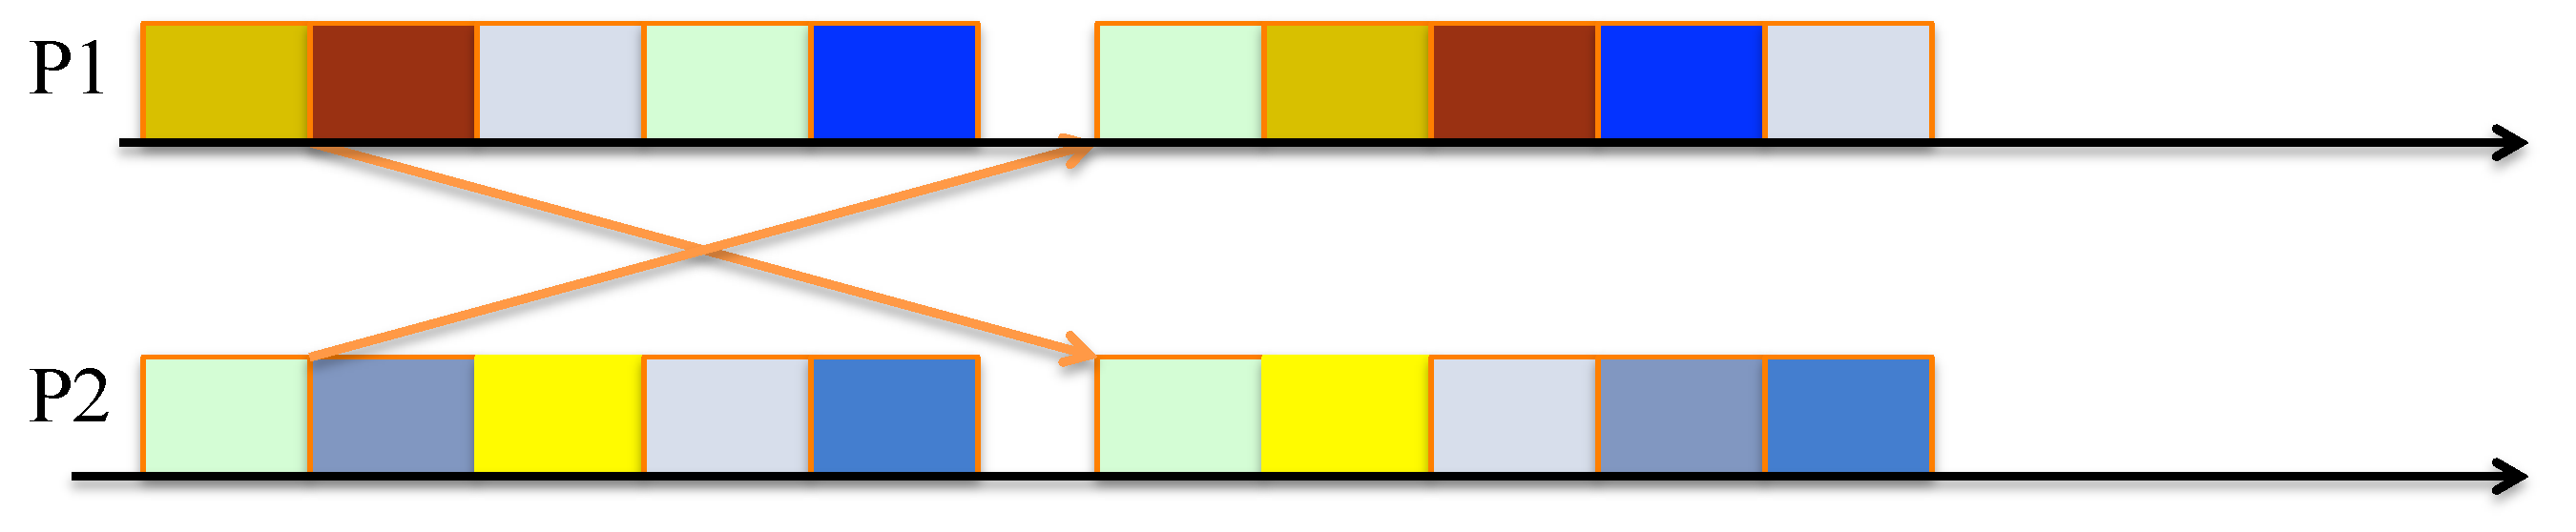
\includegraphics[width=\textwidth]{figures/stencil_timeline2} \end{center}
  \begin{center} Stencil in Charm: Communication of a chare overlaps with
  computation of others \end{center}
\end{frame}

\begin{frame}[t]
\frametitle{Modularity and Compositionality}
Without message-driven execution (and virtualization), you get either: Space-division

  \begin{center} 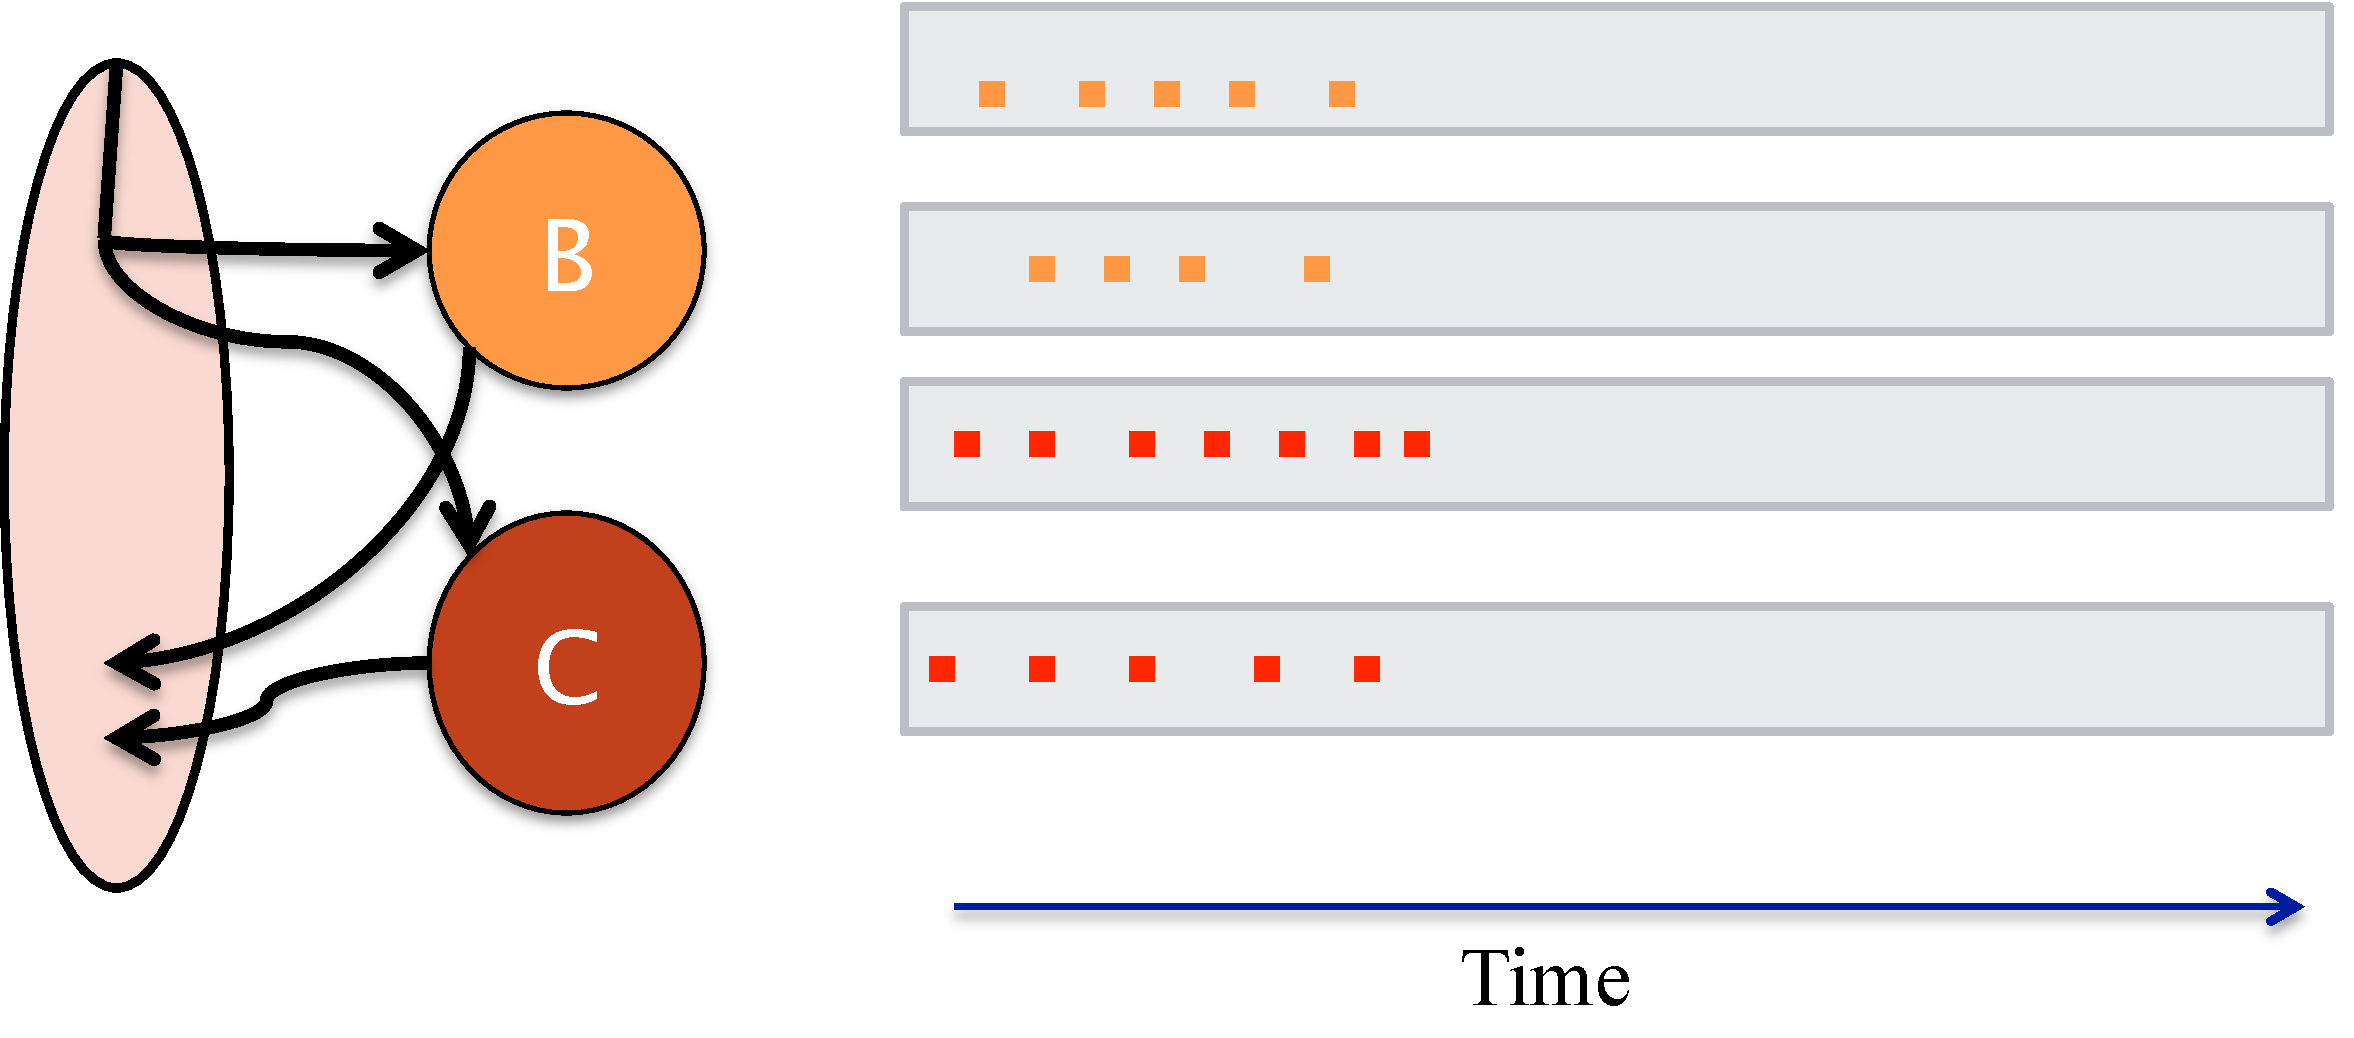
\includegraphics[width=\textwidth]{figures/stencil_space} \end{center}
\end{frame}

\begin{frame}[t]
\frametitle{Modularity and Compositionality}
Sequentialization

  \begin{center} 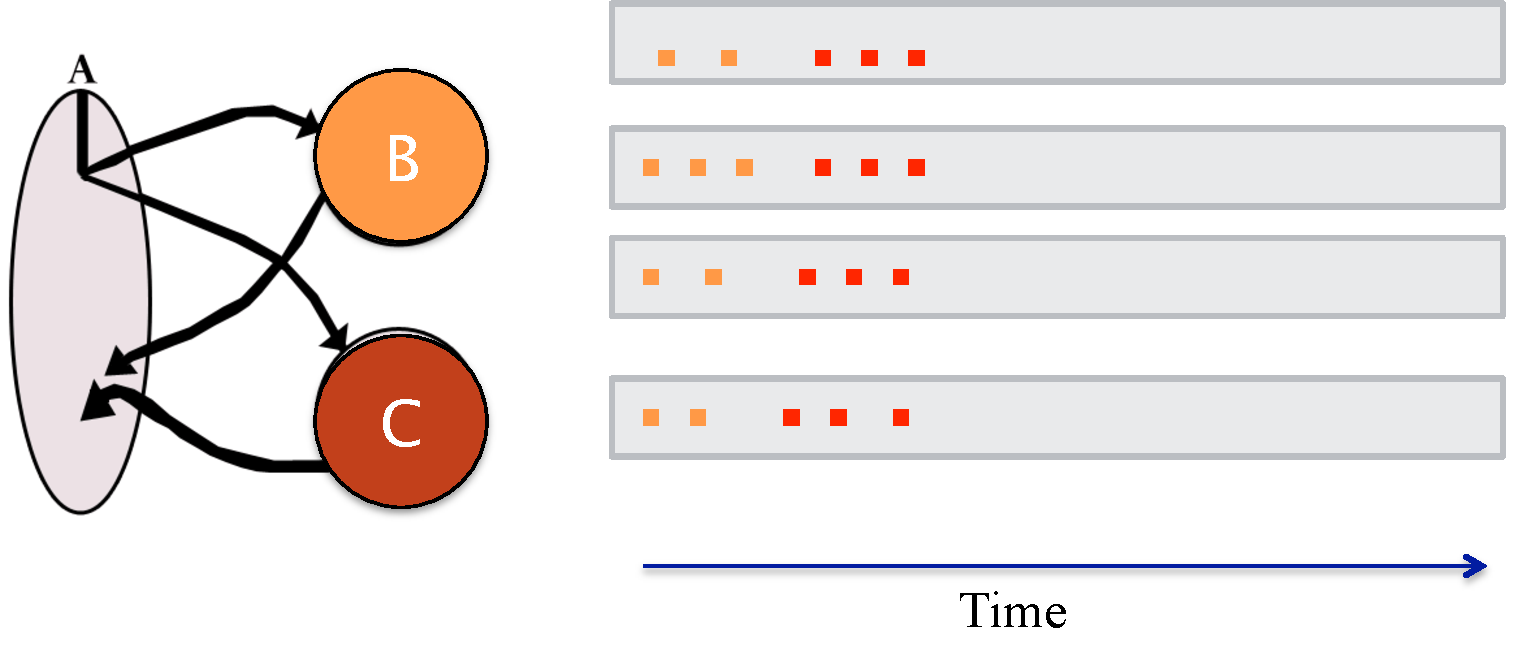
\includegraphics[width=\textwidth]{figures/stencil_seq} \end{center}
\end{frame}

\begin{frame}[t]
\frametitle{Modularity and Compositionality}
Parallel Composition: A1; (B || C ); A2
  \begin{center} 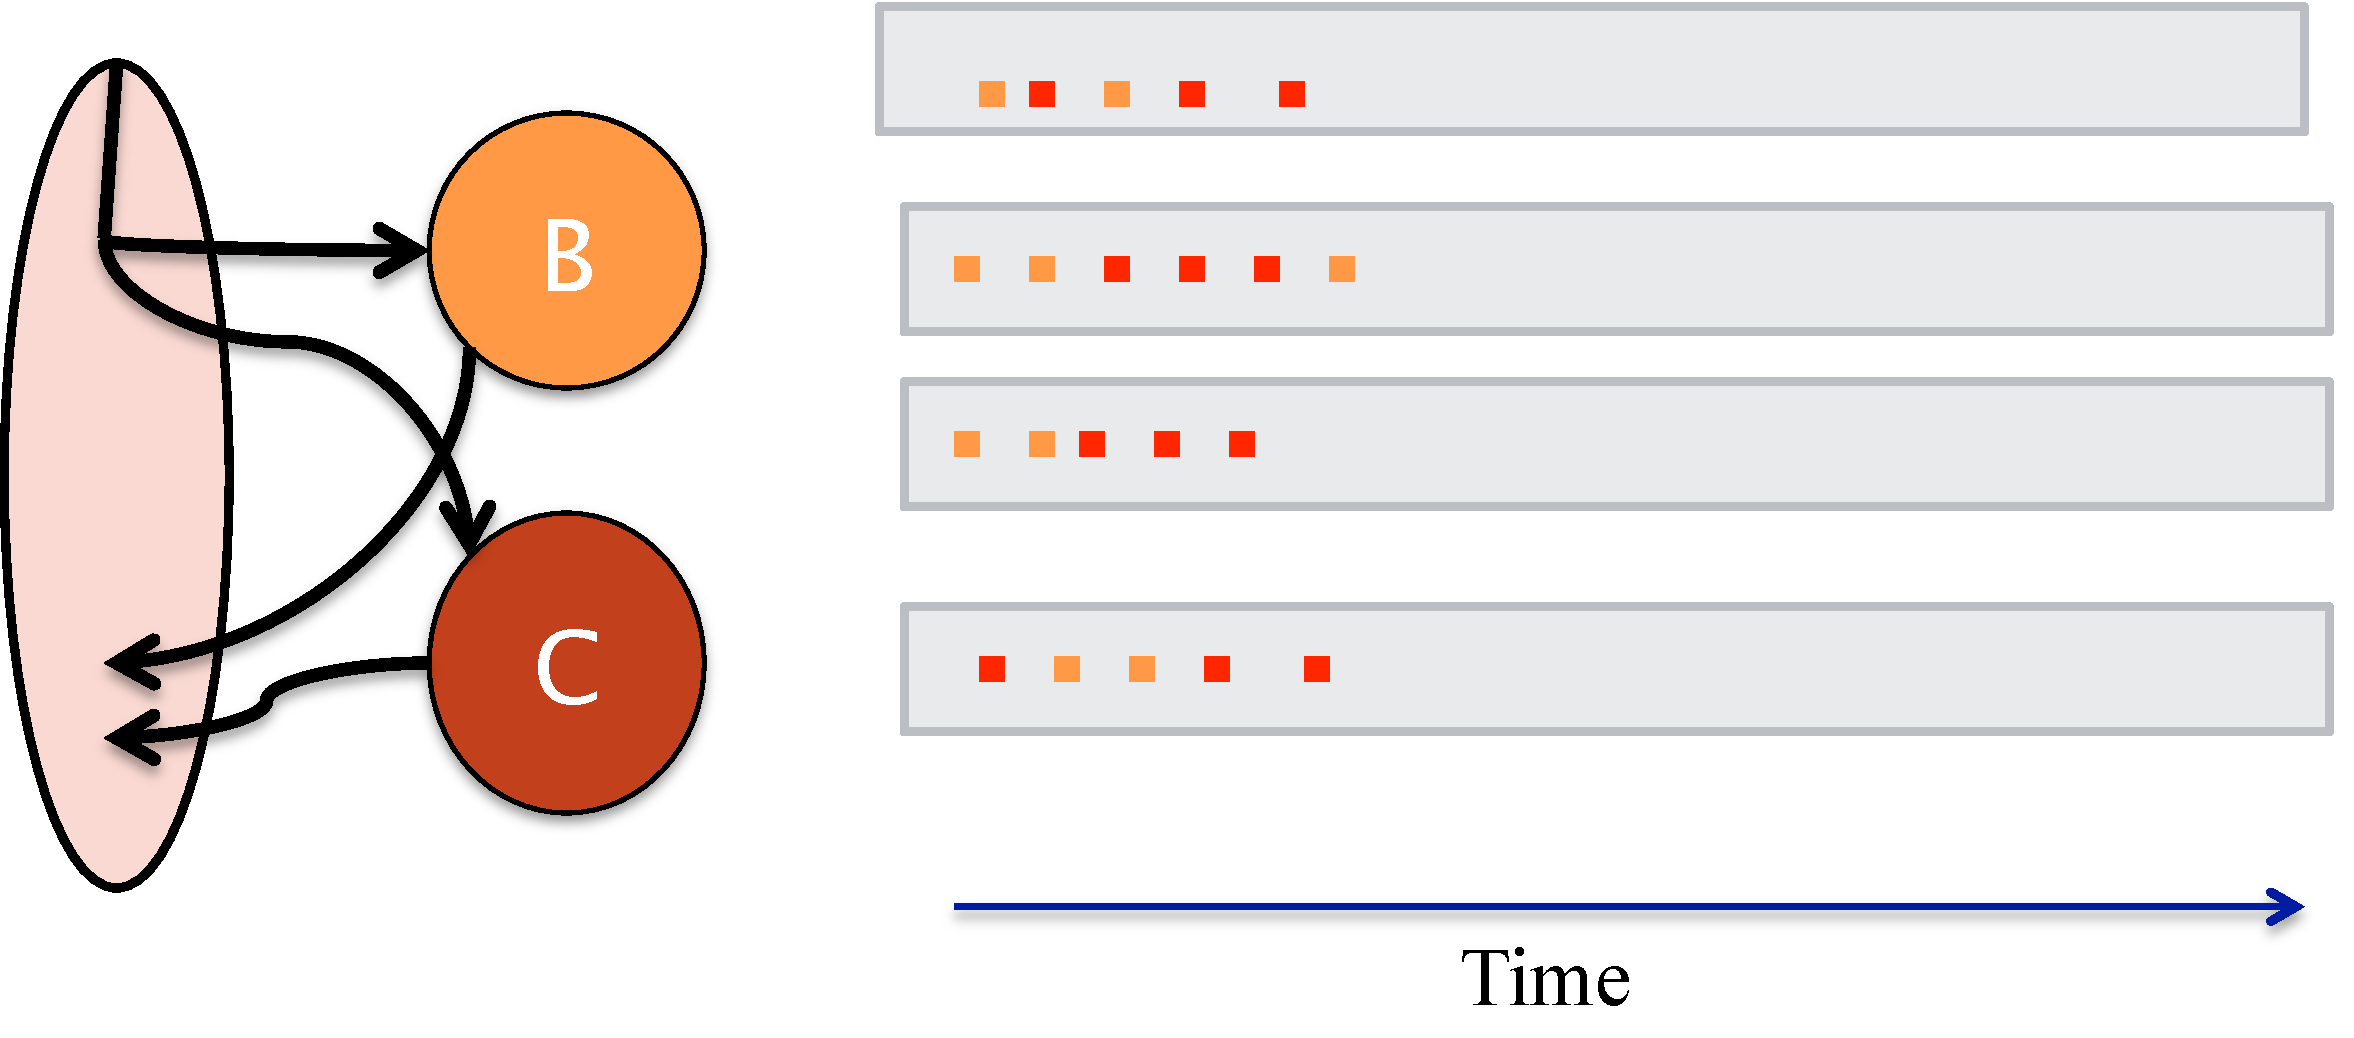
\includegraphics[width=\textwidth]{figures/stencil_charm} \end{center}
Recall: Different modules, written in different languages/paradigms, can overlap
in time and on processors, without programmer having to worry about this
explicitly

\end{frame}

%this is covered in design examples case studies section
%\begin{frame}[t]
%\frametitle{MD Parallelization Using Charm++}
%The computation is decomposed into ``natural'' objects of the application, which
%are assigned to processors by Charm++ RTS
%  \begin{center} 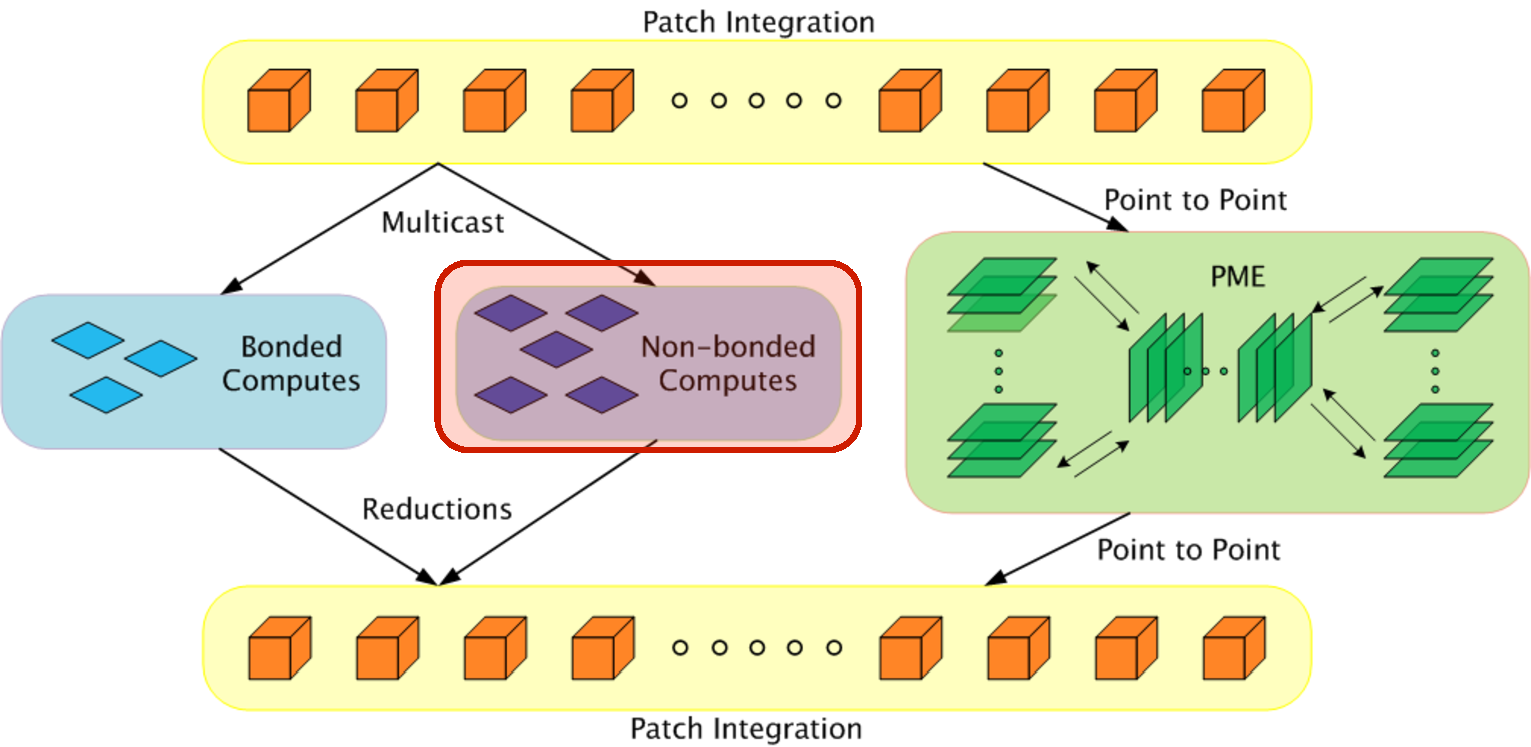
\includegraphics[width=\textwidth]{figures/md_parallelize.pdf}% \end{center}
%\end{frame}

\begin{frame}[t]
\frametitle{Migratability}
  \begin{itemize}
    \item Once the programmer has written the code without reference to
        processors, all of the communication is expressed among objects
    \item The system is free to migrate the objects across processors as and when it pleases
      \begin{itemize}
        \item It must ensure it can deliver method invocations to the objects, whereever they go
        \item This migratability turns out to be a key attribute for empowering an adaptive runtime system
      \end{itemize}
  \end{itemize}
\end{frame}

% TODO: fill in these slides
%\begin{frame}[t]
%  \frametitle{Load Balancing}
%\end{frame}

%\begin{frame}[t]
%  \frametitle{Automatic Overlap of Communication and Computation}
%\end{frame}

%\begin{frame}[t]
%  \frametitle{Fault Tolerance}
%\end{frame}

\begin{frame}[t]
\frametitle{Decomposition Independent of numCores}
  \begin{columns}
    \column{.7\textwidth}
    \begin{itemize}
      \item Rocket simulation under traditional MPI
    \end{itemize}
    \begin{center} 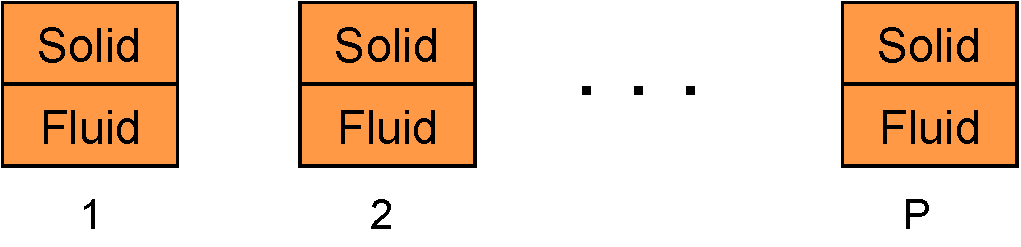
\includegraphics[width=.6\textwidth]{figures/rocket_mpi} \end{center}
    \pause
    \begin{itemize}
      \item Rocket simulation with migratable objects
      \begin{center} 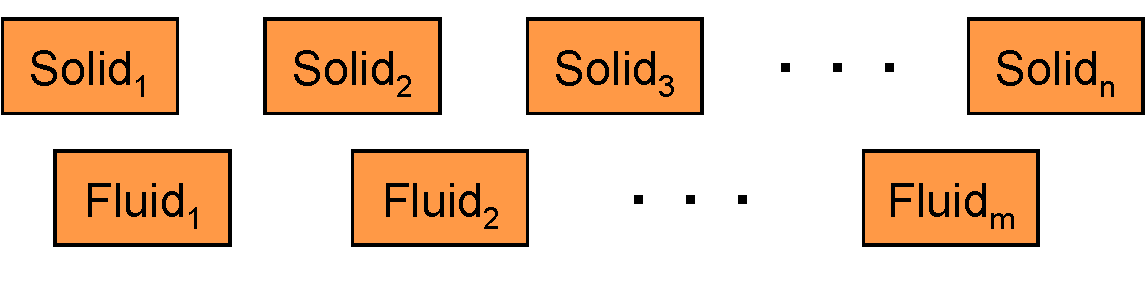
\includegraphics[width=.6\textwidth]{figures/rocket_charm} \end{center}
      \begin{itemize}
        \item Benefits: load balance, communication optimizations, modularity
      \end{itemize}
    \end{itemize}
    \onslide<1-> {
    \column{.3\textwidth}
    \vfill
    \begin{center} \includegraphics<0->[width=\textwidth]{figures/rocket.png} \end{center}
    \vfill
    }
  \end{columns}
\end{frame}

\begin{frame}[t]
\frametitle{Utility for Multi-cores, Many-cores, Accelerators}
  \begin{itemize}
    \item Objects connote and promote locality
    \item Message-driven execution is
    \begin{itemize}
      \item A strong principle of prediction for data and code use
      \item Much stronger than principle of locality
      \begin{itemize}
        \item Can be used to scale memory wall
        \item Prefetching of needed data, e.g, into scratch pad memories
      \end{itemize}
    \end{itemize}
  \end{itemize}
  \begin{center} 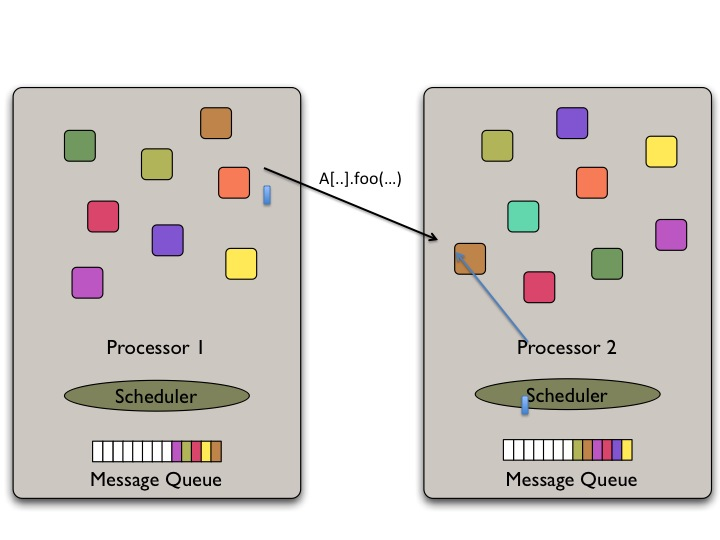
\includegraphics[width=0.6\textwidth]{figures/schedulerInvocation} \end{center}
\end{frame}

\begin{frame}[fragile]
\frametitle{Load Balancing}
\begin{itemize}
 \item Static
   \begin{itemize}
   \item Irregular applications
   \item Programmer shouldn't have to figure out ideal mapping
   \end{itemize}
 \item Dynamic
   \begin{itemize}
   \item Applications are increasingly using adaptive strategies
   \item Abrupt refinements
   \item Continuous migration of work: e.g. particles in MD
   \end{itemize}
 \item Challenges
   \begin{itemize}
   \item Performance limited by most overloaded processor
   \item The chance that one processor is severely overloaded gets higher as
     \#processors increases
   \end{itemize}
\end{itemize}
\begin{center}\textbf{Migratable Objects Empower Automated Load Balancing!}\end{center}
\end{frame}


% \begin{frame}[fragile]
% \frametitle{Principle of Persistence}
% \begin{itemize}
%  \item Once the computation is expressed in terms of its natural (migratable)
%    objects
%  \item Computational loads and communication patterns \emph{tend to} persist,
%    even in dynamic computations
%  \item So, recent past is a good predictor of near future
%  \item The runtime system mediates communication between objects, and schedules
%    execution of objects, so it can introspect: record computation loads and
%    communication graphs
% \end{itemize}
% \end{frame}


\begin{frame}[fragile]
\frametitle{A quick Example}
\framesubtitle{Weather Forecasting in BRAMS}
\begin{itemize}
 \item Brams: Brazillian weather code (based on RAMS)
 \item AMPI version (Eduardo Rodrigues, with Mendes and J. Panetta)
\end{itemize}
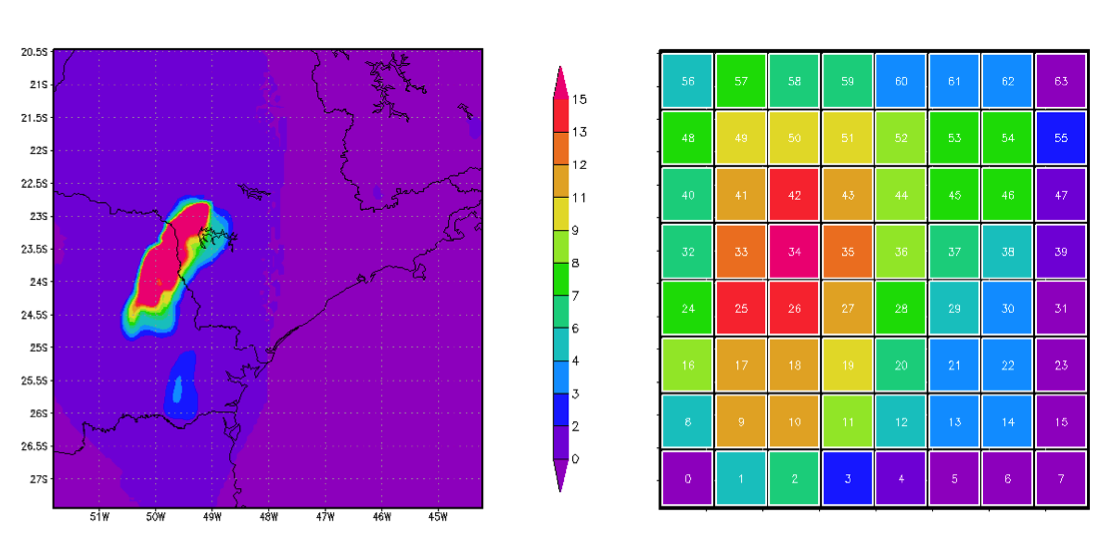
\includegraphics[width=0.9\textwidth]{figures/bramsVisual.png}
\end{frame}


\begin{frame}[fragile]
\frametitle{Basic Virtualization of BRAMS}
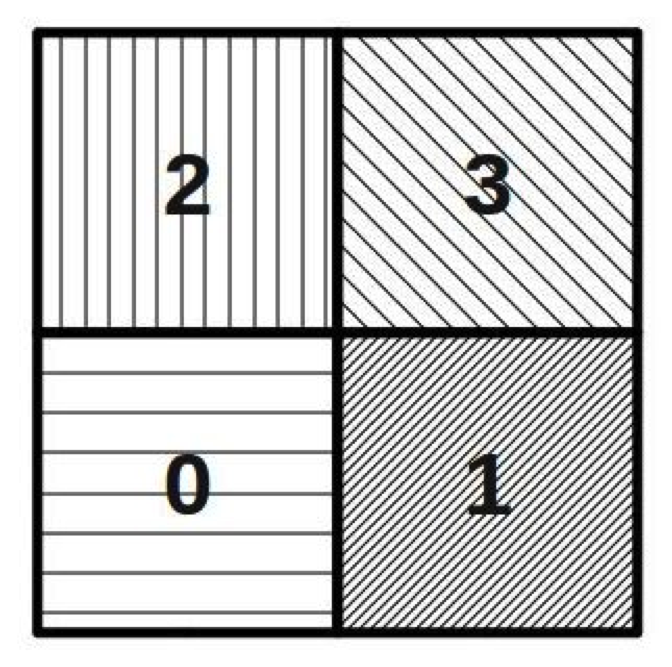
\includegraphics[width=0.5\textwidth]{figures/bramsNonVirtual.png}%
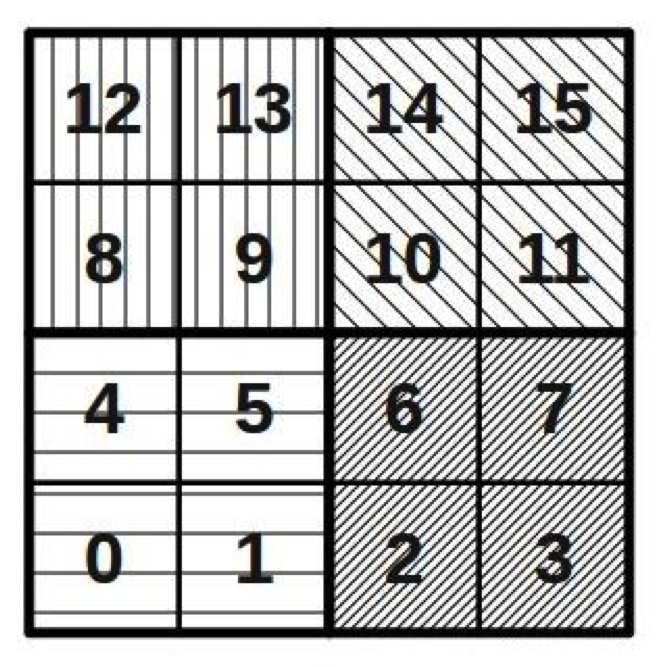
\includegraphics[width=0.5\textwidth]{figures/bramsVirtual.png}
\end{frame}

\begin{frame}[fragile]
\frametitle{Baseline: 64 objects on 64 processors}
\begin{center}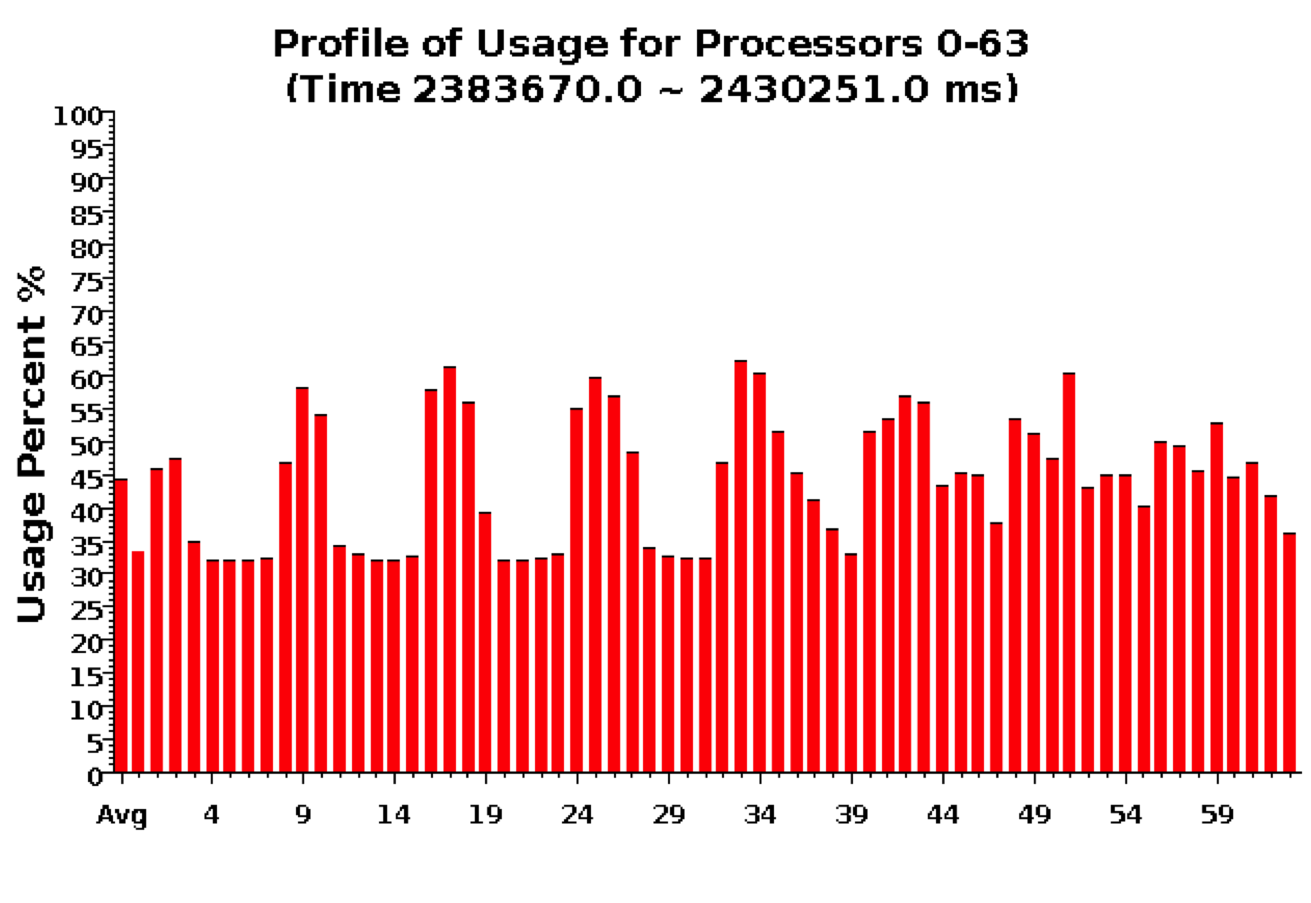
\includegraphics[width=0.9\textwidth]{figures/usageNonVirtual.png}\end{center}
\end{frame}

\begin{frame}[fragile]
\frametitle{Over-decomposition: 1024 objects on 64 processors}
\framesubtitle{Benefits from communication/computation overlap}
\begin{center}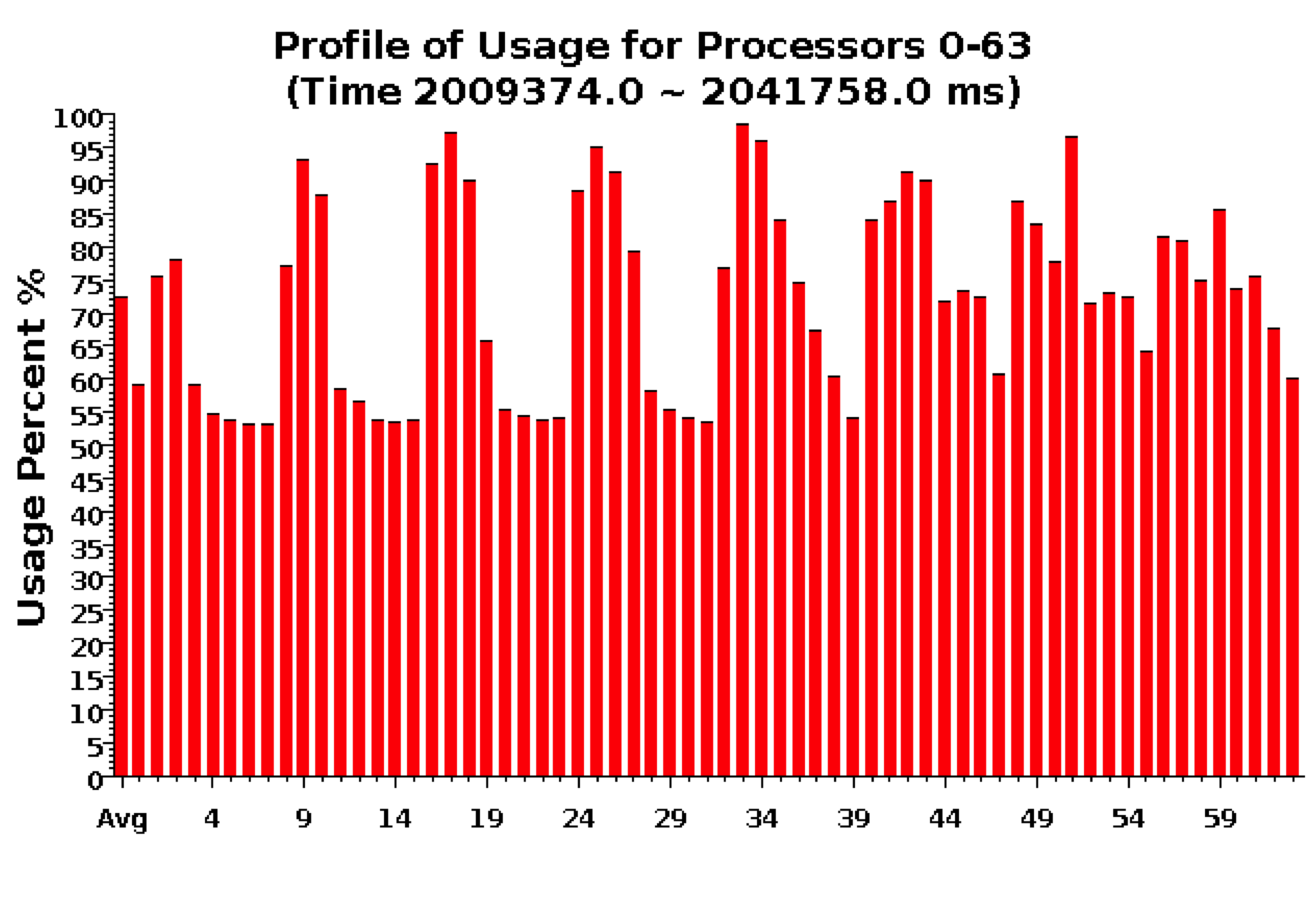
\includegraphics[width=0.9\textwidth]{figures/usageVirtual.png}\end{center}
\end{frame}

\begin{frame}[fragile]
\frametitle{With Load Balancing: 1024 objects on 64 processors}
\begin{center}
\begin{itemize}
\item No overdecomp (64 threads): 4988 sec
\item Overdecomp into 1024 threads: 3713 sec
\item Load balancing (1024 threads): 3367 sec
\end{itemize}
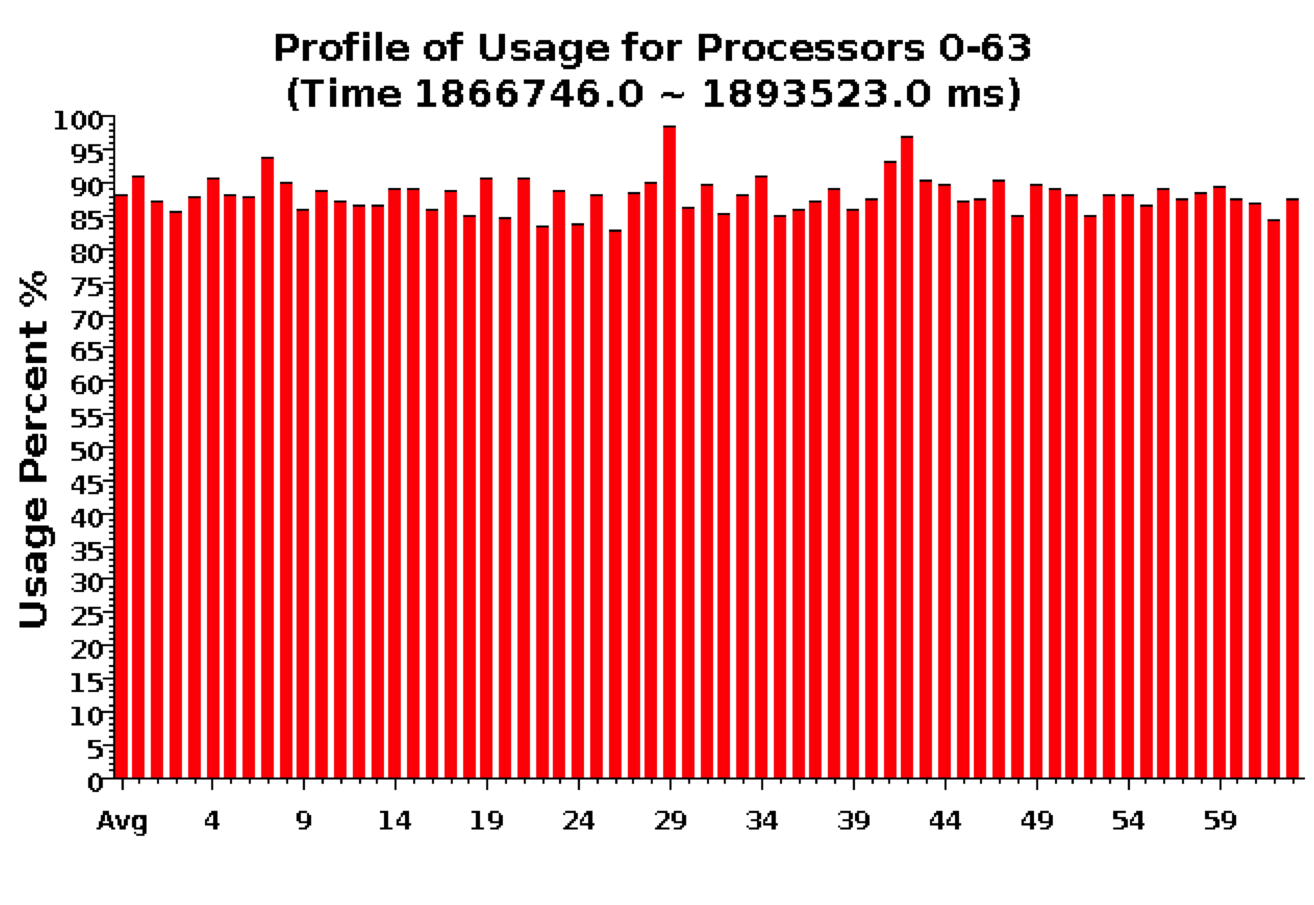
\includegraphics[width=0.8\textwidth]{figures/usageLB.png}
\end{center}
\end{frame}

\begin{frame}[fragile]
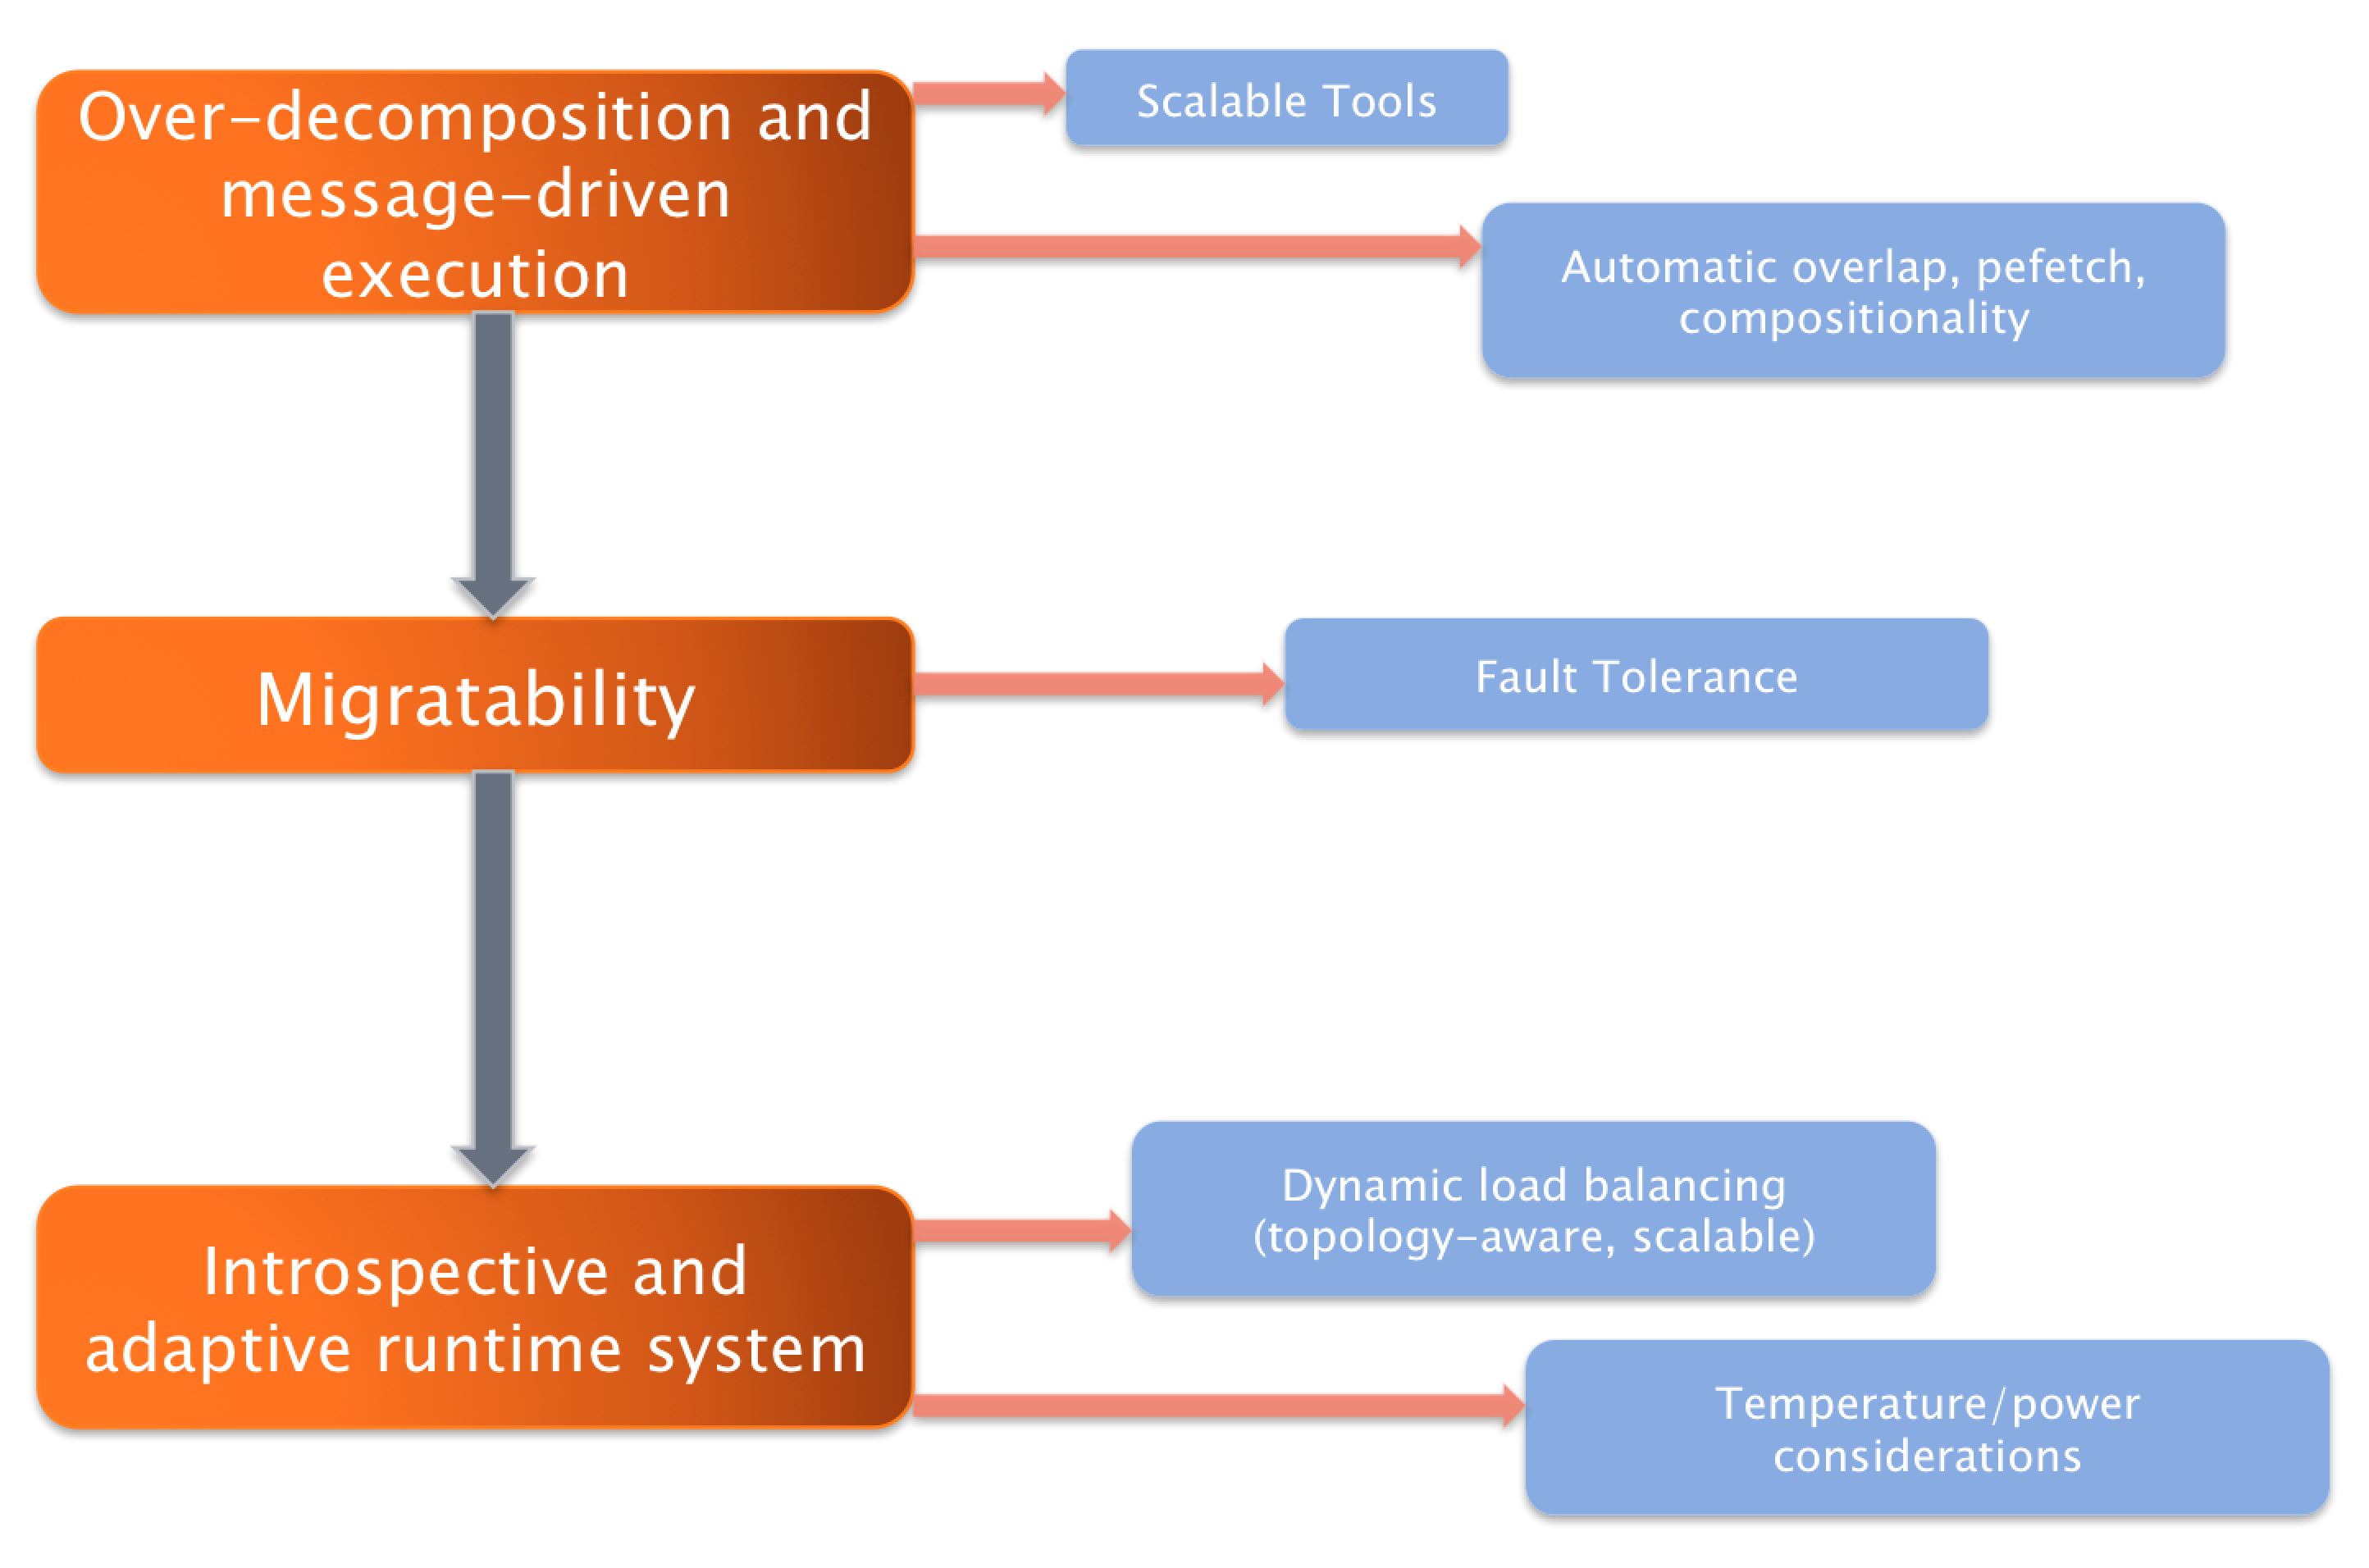
\includegraphics[width=0.9\textwidth]{figures/charmOutline.png}
\end{frame}


